\hypertarget{cv:analisisSol
	ucion}{
	\chapter{Análisis de la Solución}
}

En el presente capítulo se describirá el proceso de análisis de la solución, para ello se debe considerar que existe una propuesta de solución, la cual fue descrita en el capítulo anterior, y que será la base para el siguiente análisis. Para llevar a cabo este análisis se debe tomar en cuenta todas aquellas características con las que debe contar el sistema, ya que estas serán la base de la cual partir. \\ 

Dentro del análisis de la solución se contemplará: \textbf{análisis de requerimientos}, \textbf{análisis de procesos} y \textbf{análisis de casos de uso}. Dichos procesos serán descritos en las siguientes secciones.

\section{Análisis de requerimientos}
A continuación se describirán los requerimientos \hyperlink{cv:funcionales}{funcionales} y \hyperlink{cv:noFuncionales}{no funcionales} con los que debe contar el sistema para su correcto desarrollo. Para la identificación de los requerimientos se utilizará la siguiente nomenclatura: 

\begin{center}
\Huge{RN / RF \textit{n}: \textit{descripción\_requerimiento}}
\end{center} 

Donde: 

\begin{itemize}
	\item RN: significa Requerimiento No Funcional
	\item RF: significa Requerimiento Funcional
	\item \textit{n}: significa número de requerimiento
	\item \textit{descripción\_requerimiento}: significa una breve descripción del requerimiento
\end{itemize}

Una vez determinada la nomenclatura para identificar a los requerimientos pasaremos a describirlos: 
\hypertarget{cv:funcionales}{\subsection{Funcionales}}

El sistema deberá:

\begin{itemize}
	\item RF1: Permitir el registro de una zona turística.
	\item RF2: Permitir el trazado de un área geográfica de interés para la zona turística.
	\item RF3: Notificar a un turista que ha ingresado a una zona turística previamente registrada y delimitada.
	\item RF4: Mostrar la información de la zona turística al turista.
	\item RF5: Mostrar los servicios turísticos de la zona al turista.
	\item RF6: Crear rutas turísticas.
\end{itemize}

\hypertarget{cv:noFuncionales}{\subsection{No funcionales}}

El sistema deberá tener: 

\begin{itemize}
	\item RN1: Alta disponibilidad.
	\item RN2: Geolocalización.
	\item RN3: Alta usabilidad
\end{itemize}

\section{Análisis de casos de uso}
Para el análisis de casos de uso se tomaron en cuenta los requerimientos funcionales y los no funcionales, descritos en la sección anterior, que fueron identificados a partir de la propuesta de solución. \\

Para poder llevar a cabo un correcto análisis de casos de uso primero se tuvo que tener bien identificados a loa actores o usuarios finales que participarán en el uso del sistema. Una vez identificados se realizó una arquitectura de solución en la cual se definieron los módulos a desarrollar para el sistema, el análisis de casos de uso parte tomando como base estos módulos ya que en ellos será donde se centre la interacción del usuario con el sistema. \\

En la Figura \ref{fig:casosDeUso} se muestra el diagrama general de los casos de uso identificados para el sistema, en él puede observarse que los casos de uso se encuentran divididos por actores y que cada uno de estos tiene un nombre.


\hypertarget{fig:casosDeUso}{
	\begin{figure}[htbp]
		\begin{center}
			\hypertarget{fig:casosDeUso}{
				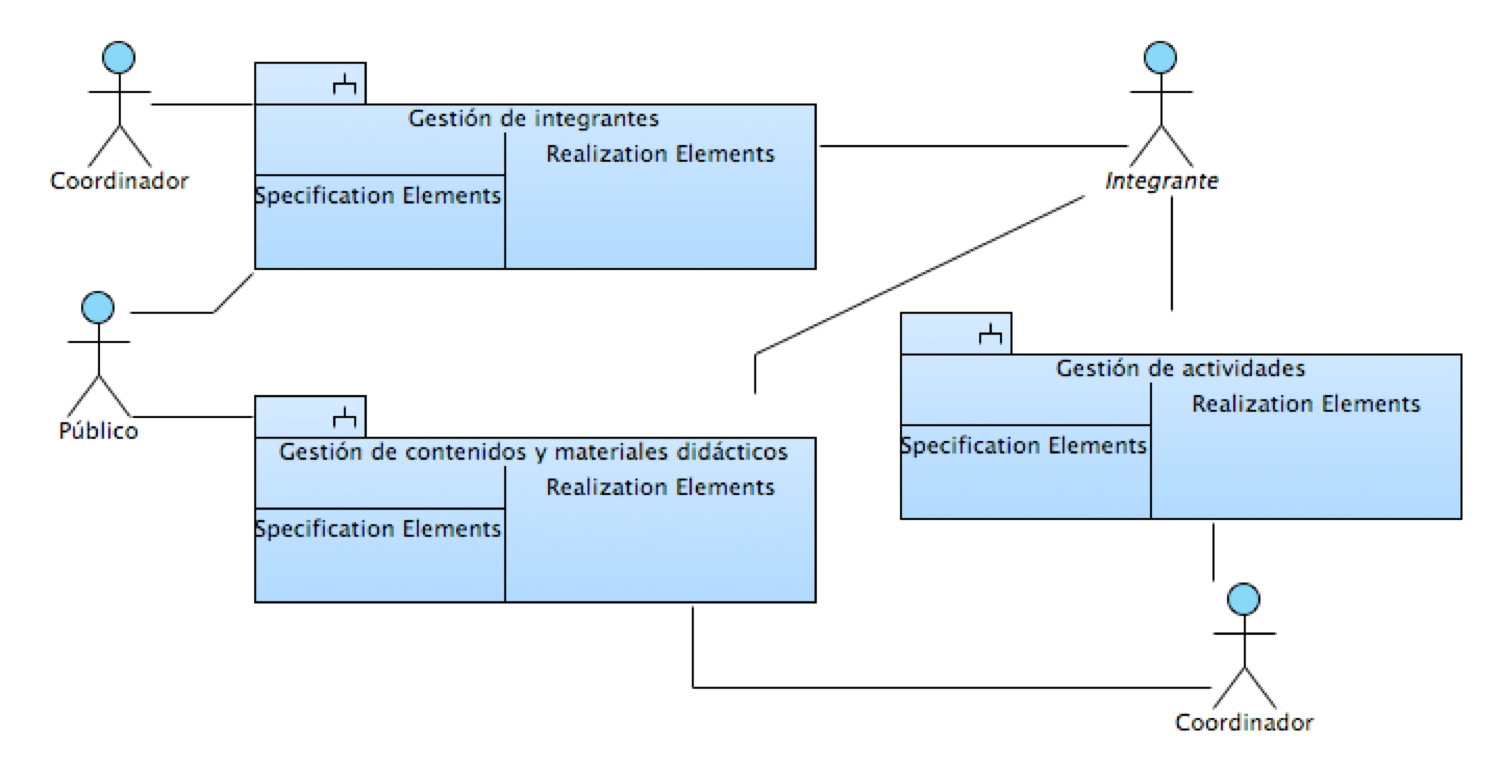
\includegraphics[angle=90, scale=.4]{casosDeUso/images/casosDeUso}
				\caption{Casos de uso}
			}
			\label{fig:casosDeUso}
		\end{center}
	\end{figure}
}

\newpage
A continuación se muestra la nomenclatura utilizada para asignar el nombre a los casos de uso:

\begin{center}
	\Huge{\textit{Iniciales\_módulo}-CU\textit{n}: \textit{nombre\_caso\_de\_uso}}
\end{center}

Donde: 

\begin{itemize}
	\item \textbf{iniciales\_módulo}: significa que son las iniciales del módulo en el que se encuentra el caso de uso, los módulos son: 
	\begin{itemize}
		\item RE: Registro
		\item LR: Localización de rutas
		\item PO: Posicionamiento
		\item II: Interacción de la información
		\item SE: Servicios
		\item IR: Información y representación de estadísticas turísticas
		\item RA: Registro de área turística
	\end{itemize}

	\item \textbf{n}: es el número de caso de uso.
	
	\item \textbf{nombre\_caso\_de\_uso}: es el nombre del caso de uso.
\end{itemize}

Para realizar la documentación se tomaron los casos de uso y se separaron por módulo. Cabe mencionar que aunque sean distintos módulos los casos de uso tienen una relación entre sí para poder construir el sistema. \\

La documentación de los casos de uso se divide en tres partes:

\begin{enumerate}
	\item Descripción
	\item Atributos
	\item Trayectorias
\end{enumerate}

La descripción es un breve resumen de lo que trata el caso de uso, en ella se describe el por qué del caso de uso, para qué es importante tenerlo, el objetivo principal y lo que se obtiene al ejecutarlo.\\

Los atributos son descritos en una tabla, esto facilita al desarrollador identificar las entradas y salidas del caso de uso, su precedencia y los cambios que produce al sistema. \\

La trayectoria son los pasos a seguir para la correcta ejecución y desarrollo del caso de uso, en esta puede haber trayectorias alternativas, puntos de extensión a otros casos de uso o inclusión de otros casos casos de uso. \\

A continuación se detallan los casos de uso:

<<<<<<< HEAD

% !TeX spellcheck = <none>
% \IUref{IUAdmPS}{Administrar Planta de Selección}
% \IUref{IUModPS}{Modificar Planta de Selección}
% \IUref{IUEliPS}{Eliminar Planta de Selección}

% 


% Copie este bloque por cada caso de uso:
%-------------------------------------- COMIENZA descripción del caso de uso.

%\begin{UseCase}[archivo de imágen]{UCX}{Nombre del Caso de uso}{
%--------------------------------------
	\begin{UseCase}{CU6}{Registrar Comentario}{
		Este caso de uso permite al usuario registrar un comentario y una puntuación a un servicio turístico seleccionado que se encuentre dentro de un área registrada. Cabe destacar que para poder acceder a este caso de uso es necesario que se valide la regla de negocio XXXXX .
	}
		\UCitem{Versión}{\color{Gray}1.0}
		\UCitem{Actor}{\hyperlink{Usuario}{Usuario}}
		\UCitem{Propósito}{Registrar un comentario y puntuación.}
		\UCitem{Entradas}{Comentario y Puntuación}
		\UCitem{Origen}{Teclado}
		\UCitem{Salidas}{N.A.}
		\UCitem{Precondiciones}{Cumplir con la regla de negocio XXXXXX}
		\UCitem{Postcondiciones}{Quedará el comentario y la puntuación, asociada al servicio turístico}
		\UCitem{Errores}{}
		\UCitem{Tipo}{Caso de uso Cuaternario}
		\UCitem{Observaciones}{}
	\end{UseCase}
%--------------------------------------
	\begin{UCtrayectoria} 
		
		\UCpaso[\UCactor] Da clic en el botón \IUbutton{Comentar} de la pantalla  \IUref{IU8}{Principal}.
		
		\UCpaso Obtiene la descripción, puntuación y los comentarios del servicio seleccionado.
		
		\UCpaso Verifica que el usuario tenga permitido comentar mediante la regla de negocio XXXXXXXXXX. \Trayref{A}.
		
		\UCpaso Despliega la pantalla \IUref{IU8}{Principal} con los datos asociados al servicio, así como habilitados los botones \IUbutton{Ver Mapa} y \IUbutton{Comentar}.
		
		\UCpaso[] Termina el caso de uso.
		
	\end{UCtrayectoria}

%--------------------------------------		
		\begin{UCtrayectoriaA}{A}{El usuario no tiene permitido realizar un comentario.}
			
		\UCpaso Despliega la pantalla \IUref{IU8}{Principal} con los datos asociados al servicio y únicamente habilitado el botón \IUbutton{Ver Mapa}.
		
		\UCpaso[] Termina el caso de uso.
		
	\end{UCtrayectoriaA}
	
	
=======
% !TeX spellcheck = <none>
% \IUref{IUAdmPS}{Administrar Planta de Selección}
% \IUref{IUModPS}{Modificar Planta de Selección}
% \IUref{IUEliPS}{Eliminar Planta de Selección}

% 


% Copie este bloque por cada caso de uso:
%-------------------------------------- COMIENZA descripción del caso de uso.

%\begin{UseCase}[archivo de imágen]{UCX}{Nombre del Caso de uso}{
%--------------------------------------
	\begin{UseCase}{CU6}{Registrar Comentario}{
		Este caso de uso permite al usuario registrar un comentario y una puntuación a un servicio turístico seleccionado que se encuentre dentro de un área registrada. Cabe destacar que para poder acceder a este caso de uso es necesario que se valide la regla de negocio XXXXX .
	}
		\UCitem{Versión}{\color{Gray}1.0}
		\UCitem{Actor}{\hyperlink{Usuario}{Usuario}}
		\UCitem{Propósito}{Registrar un comentario y puntuación.}
		\UCitem{Entradas}{Comentario y Puntuación}
		\UCitem{Origen}{Teclado}
		\UCitem{Salidas}{N.A.}
		\UCitem{Precondiciones}{Cumplir con la regla de negocio XXXXXX}
		\UCitem{Postcondiciones}{Quedará el comentario y la puntuación, asociada al servicio turístico}
		\UCitem{Errores}{}
		\UCitem{Tipo}{Caso de uso Cuaternario}
		\UCitem{Observaciones}{}
	\end{UseCase}
%--------------------------------------
	\begin{UCtrayectoria} 
		
		\UCpaso[\UCactor] Da clic en el botón \IUbutton{Comentar} de la pantalla  \IUref{IU8}{Principal}.
		
		\UCpaso Obtiene la descripción, puntuación y los comentarios del servicio seleccionado.
		
		\UCpaso Verifica que el usuario tenga permitido comentar mediante la regla de negocio XXXXXXXXXX. \Trayref{A}.
		
		\UCpaso Despliega la pantalla \IUref{IU8}{Principal} con los datos asociados al servicio, así como habilitados los botones \IUbutton{Ver Mapa} y \IUbutton{Comentar}.
		
		\UCpaso[] Termina el caso de uso.
		
	\end{UCtrayectoria}

%--------------------------------------		
		\begin{UCtrayectoriaA}{A}{El usuario no tiene permitido realizar un comentario.}
			
		\UCpaso Despliega la pantalla \IUref{IU8}{Principal} con los datos asociados al servicio y únicamente habilitado el botón \IUbutton{Ver Mapa}.
		
		\UCpaso[] Termina el caso de uso.
		
	\end{UCtrayectoriaA}
	
	
% !TeX spellcheck = <none>
% \IUref{IUAdmPS}{Administrar Planta de Selección}
% \IUref{IUModPS}{Modificar Planta de Selección}
% \IUref{IUEliPS}{Eliminar Planta de Selección}

% 


% Copie este bloque por cada caso de uso:
%-------------------------------------- COMIENZA descripción del caso de uso.

%\begin{UseCase}[archivo de imágen]{UCX}{Nombre del Caso de uso}{
%--------------------------------------
	\begin{UseCase}{CU6}{Registrar Comentario}{
		Este caso de uso permite al usuario registrar un comentario y una puntuación a un servicio turístico seleccionado que se encuentre dentro de un área registrada. Cabe destacar que para poder acceder a este caso de uso es necesario que se valide la regla de negocio XXXXX .
	}
		\UCitem{Versión}{\color{Gray}1.0}
		\UCitem{Actor}{\hyperlink{Usuario}{Usuario}}
		\UCitem{Propósito}{Registrar un comentario y puntuación.}
		\UCitem{Entradas}{Comentario y Puntuación}
		\UCitem{Origen}{Teclado}
		\UCitem{Salidas}{N.A.}
		\UCitem{Precondiciones}{Cumplir con la regla de negocio XXXXXX}
		\UCitem{Postcondiciones}{Quedará el comentario y la puntuación, asociada al servicio turístico}
		\UCitem{Errores}{}
		\UCitem{Tipo}{Caso de uso Cuaternario}
		\UCitem{Observaciones}{}
	\end{UseCase}
%--------------------------------------
	\begin{UCtrayectoria} 
		
		\UCpaso[\UCactor] Da clic en el botón \IUbutton{Comentar} de la pantalla  \IUref{IU8}{Principal}.
		
		\UCpaso Obtiene la descripción, puntuación y los comentarios del servicio seleccionado.
		
		\UCpaso Verifica que el usuario tenga permitido comentar mediante la regla de negocio XXXXXXXXXX. \Trayref{A}.
		
		\UCpaso Despliega la pantalla \IUref{IU8}{Principal} con los datos asociados al servicio, así como habilitados los botones \IUbutton{Ver Mapa} y \IUbutton{Comentar}.
		
		\UCpaso[] Termina el caso de uso.
		
	\end{UCtrayectoria}

%--------------------------------------		
		\begin{UCtrayectoriaA}{A}{El usuario no tiene permitido realizar un comentario.}
			
		\UCpaso Despliega la pantalla \IUref{IU8}{Principal} con los datos asociados al servicio y únicamente habilitado el botón \IUbutton{Ver Mapa}.
		
		\UCpaso[] Termina el caso de uso.
		
	\end{UCtrayectoriaA}
	
	
>>>>>>> 4b243b0421e3340fd688e8e3a78460d652bbf8cd

